\documentclass[a4paper]{article}

\usepackage[english]{babel}
%\usepackage[utf8]{inputenc}
\usepackage{amsmath}
\usepackage{graphicx}

\usepackage{natbib}
\usepackage{fixltx2e}
\usepackage[version=3]{mhchem}
\usepackage{float}

\usepackage{titlesec}
\usepackage{titling}
\usepackage{fontspec}
\usepackage{authoraftertitle}

\setmainfont{Lato} 
\setsansfont{Trebuchet MS} 
\setmonofont{Inconsolata} 
% Specify different font for section headings
\newfontfamily\headingfont[]{Georgia}
\titleformat*{\section}{\LARGE\headingfont}
\titleformat*{\subsection}{\Large\headingfont}
\titleformat*{\subsubsection}{\large\headingfont}
\renewcommand{\maketitlehooka}{\headingfont}

\bibliographystyle{agsm}

\title{Devonian Granite Types in Victoria and their Origin}

\author{James Stone - 761353 \thanks{ERTH10002 Understanding Planet Earth -  Dr Anne-Marie Tosolini and Prof David Phillips}}

\date{October 2015}

\begin{document}
\maketitle
\newpage

\begin{abstract}
Granite can be geochemically classified by its source; Sedimentary (S-type) or Igneous (I-type). 
Another method of classification is based on magma temperature.

Victorian granites within the Lachlan Fold Belt are predominantly S-type to the west and I-type to the east. An explanation for this observation is that the Lachlan Fold Belt accreted onto the older Gondwanan Craton to the west during the Benambran Orogeny, leading to the Devonian granite development.
\end{abstract}

\section{Introduction}

The granites of Victoria are situated almost totally within the Lachlan Fold Belt, (or Orogen), See Figure~\ref{fig:VicMapRockTypes} and Figure~\ref{fig:SEAustraliaOrdovicianTerrannes}. The regional geological environment through which the Devonain granites intruded is one of alternating deep and shallow marine sedimentary rock deposited during the Ordovician and Silurian along the continental edge of the older Delamerian Orogen to the West.

Classification of granites by origin was originally pioneered by Chappell and White in 1974 and was initially specific to the Berridale (I-type) batholith and the Kosciuszko (S-type) batholith in Southern New South Wales. Whilst this was regionally limiting, their research and conclusions have largely stood the test of time and have since been applied with success to describe granite emplacement mechanisms throughout the Lachlan Fold Belt and across other granitic regions of the world.

\section{Granite Types}

Granites can be classified into two major types; the S-type and the I-type, \cite{BWChappell}. This classification distinguishes the granites by their source and utilises both geochemical and petrological characteristics. It is accepted that the present day features of granites form an "image" of their source rocks, \cite{hine1978contrasts}, acknowledging that fractionation of the magma body often occurs. The more homogeneous the batholith, the more it accurately reveals its origins. 

Additionally, the more mafic the granite, the closer it resembles its source rocks, and the easier it can be classified into S and I-type. If a granite is more felsic, this distinction is harder.   


\begin{figure}[H]
\centering
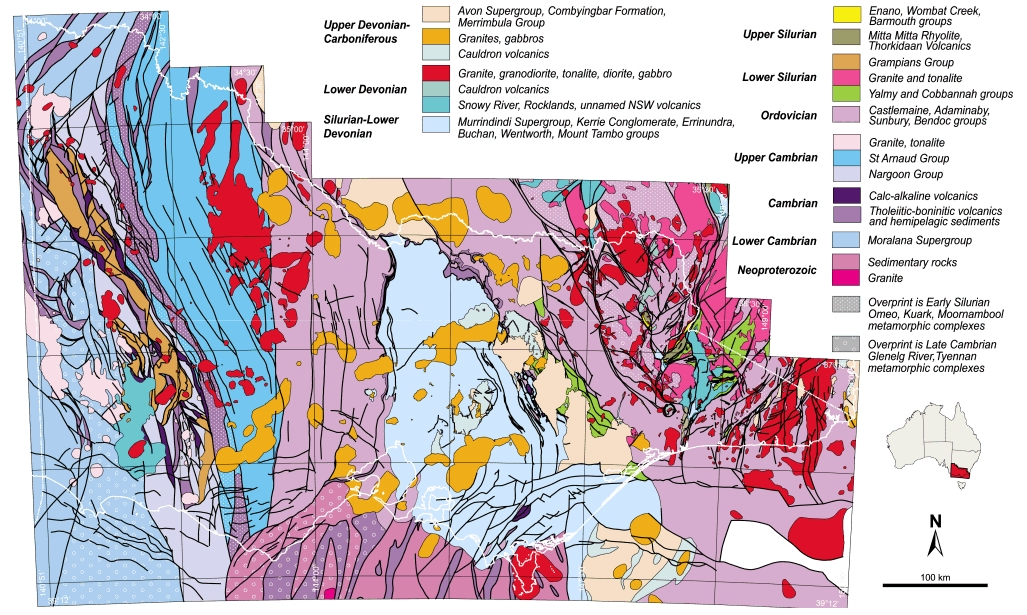
\includegraphics[width=1\textwidth]{vicmaprocktypes.jpg}
\caption{\label{fig:VicMapRockTypes}Geological Map of Victoria From: \cite{vandenberg2000tasman}}
\end{figure}

\subsection{S and I-types}

\subsubsection{S-type}
S-type granites are composed of sedimentary rocks that have undergone anatexis. Chappell and White, (1984) describes these sources as \textit{supracrustal}.
Petrologically, they are more likely to contain meta-sedimentary xenoliths. S-type granites have a chemical composition that is relatively higher in sodium and calcium. It is thought that this distinction is the result of calcium enrichment in carbonate and calcareous sediments and sodium enrichment through concentration of salt water and subsequent evaporation and capture as evaporitic sediments. 

\subparagraph{Chemical Composition:}

\ce{Na2O} \textgreater 3.2\% in more felsic granites\newline
\ce{Na2O} \textgreater 2.2\% in more mafic granites\newline
This can be seen in Figure~\ref{fig:SodiumPotassium}.\newline\newline
Mol. \ce{Al2O3 / ( Na2O + K2O + CaO)} \textless 1.1 see Figure  ~\ref{fig:AluminiumSaturationIndex} \newline

\subsubsection{I-type}
I-types granites are derived from igneous source material. Chappell and White describe these sources as being generally \textit{infracrustal}. Petrologically, they often contain mafic hornblende-bearing xenoliths.

\subparagraph{Chemical Composition:}

\ce{Na2O} \textless 3.2\% in more felsic granites. \newline
\ce{Na2O} \textless 2.2\% in more mafic granites. \newline
This can be seen in Figure~\ref{fig:SodiumPotassium}.\newline\newline
Mol. \ce{Al2O3 // ( Na2O + K2O + CaO)} \textgreater 1.1 on the Aluminium Saturation Index, see Figure  ~\ref{fig:AluminiumSaturationIndex}. 

\begin{figure}[H]
\centering
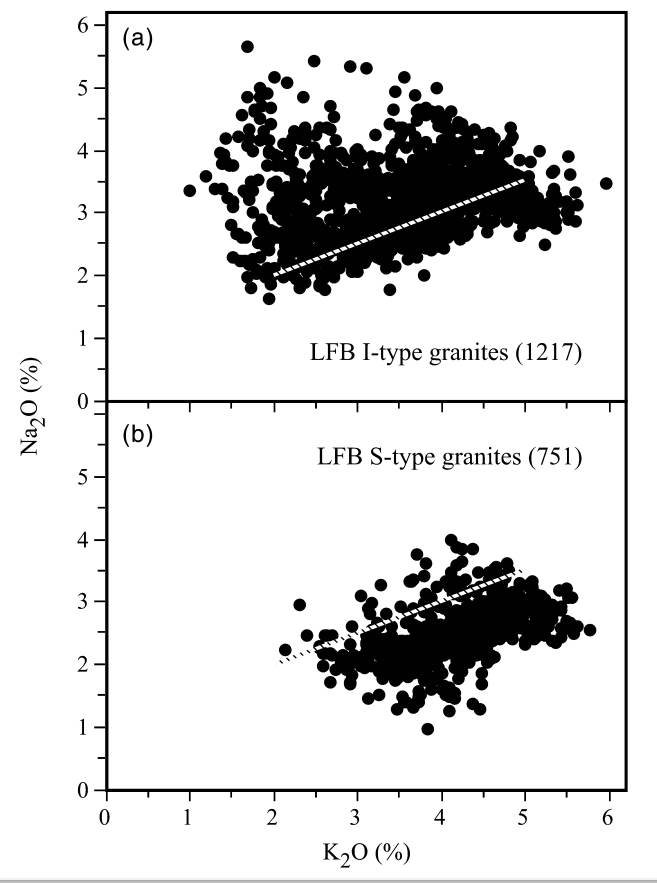
\includegraphics[width=1\textwidth]{SodiumPotassium.jpg}
\caption{\label{fig:SodiumPotassium} \ce{Na2O} vs \ce{K2O}. The dotted line on both plots (I-type vs S-type) shows the border chosen to distinguish the two types  From: \cite{chappell2001two}}
\end{figure}

\subsection{High and Low Temperature Granites}
Because felsic granites have similar major element geochemistry, a newer classification for the granites of Victoria has been proposed by \cite{chappell2010high} which is magmatic temperature based. This classification utilises trace element geochemistry. As an example, S-type granites have high P and low Th and Ce in relative abundance, compared to I-types \cite{chappell1998high}. Despite this classification system being different to S and I-type granites, the higher temperature granites are generally classified as A type granites (felsic composition) or I-type granites (mafic composition). Lower temperature granites being classified as S-type and the remaining are I-type granites. These comprise \textasciitilde 90 \% of the Lachlan fold belt. \cite{chappell2001two}

As S-type granites are low in \ce{Na} and \ce{Ca} they are over saturated in \ce{Al}. As a result of this, when Chappell and White were determining the boundary they realised they had created a distinction between S and I-types also on Aluminium Saturation - see Figure  ~\ref{fig:AluminiumSaturationIndex}.

\begin{figure}[H]
\centering
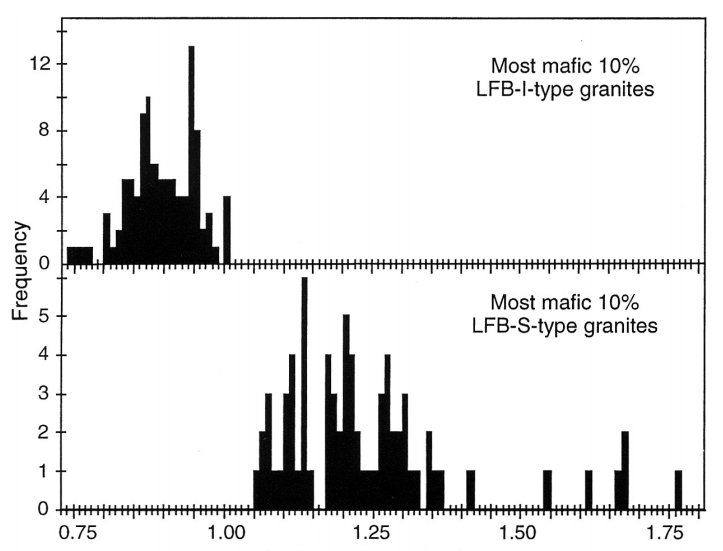
\includegraphics[width=1\textwidth]{Aluminium_Saturation_Index.jpg}
\caption{\label{fig:AluminiumSaturationIndex}Aluminium Saturation Index of Granites from Lachlan Fold Belt. From: \cite{chappell1998high}}
\end{figure}

\section{The Geological Setting}

It is evident that, in a general sense, the present day location of S-type granites in Victoria, (and the Lachlan Fold Belt) is further to the west than I-type granites. This supports the theory that the sedimentary source of the S-types is the continental crust of the older Pre-Cambrian Delamerian Fold Belt sediments which immediately underlay the Lachlan Fold Belt to the West. The predominance of I-type granites further to the east also supports the theory that in this location, there was less shallow crustal and more deeper crustal, shallow mantle involvement.

\begin{figure}[H]
\centering
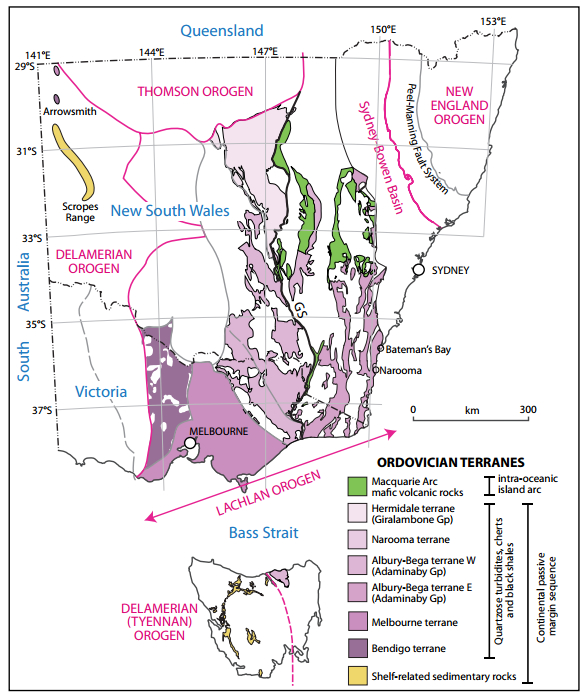
\includegraphics[width=1\textwidth]{SEAustraliaOrdovicianTerrannes.jpg}
\caption{\label{fig:SEAustraliaOrdovicianTerrannes}South Eastern Australia Ordovician Terrranes From: \cite{aitchison2012accordion}}
\end{figure}

During the early Ordovician, (ca. 430Ma), the Benambran Orogeny resulted in the accretion of the intra-oceanic Macquarie Arc to the Gondwana Plate, \cite{BenambranOrogeny}.  During this period, the Panthalassan Oceanic plate subducted under Gondwana, as depicted in Figure~\ref{fig:GraniteModels} and Figure~\ref{fig:SEAustraliaOrdovicianTerrannes} (structural  terrane map). There are two models described in this diagram, the Retreating Accretionary Orogen "Accordian" Model and the Subduction Flip Model, \cite{aitchison2012accordion}. Importantly, both models satisfy the requirement for S-type sedimentary sourced granites closer to the Gondwanan margin and I-type granites further East.

\begin{figure}[H]
\centering
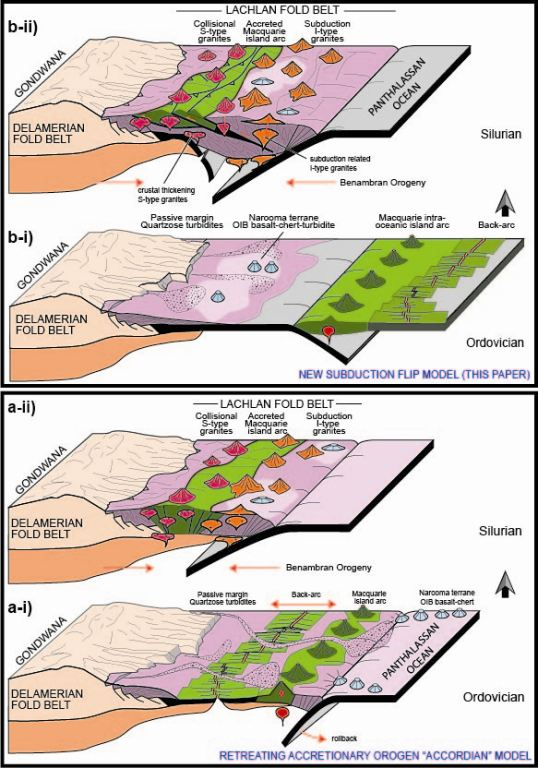
\includegraphics[width=1\textwidth]{granite_models.jpg}
\caption{\label{fig:GraniteModels} Possible Geological Settings of the Lachlan Fold Belt and origin of its Devonian granites. From: \cite{aitchison2012accordion}}
\end{figure}


Typical ages of granites within the Victorian Lachlan Fold Belt are from 340 to 440Ma, see  Figure~\ref{fig:GraniteTypes}. These generally occurred during the Devonian, (359 to 419 Ma). It is evident that it took up to 90My for the effects of the Benambran Orogeny to heat up the source rock enough for it to become mobilised in the crust to form granites.


\begin{figure}[H]
\centering
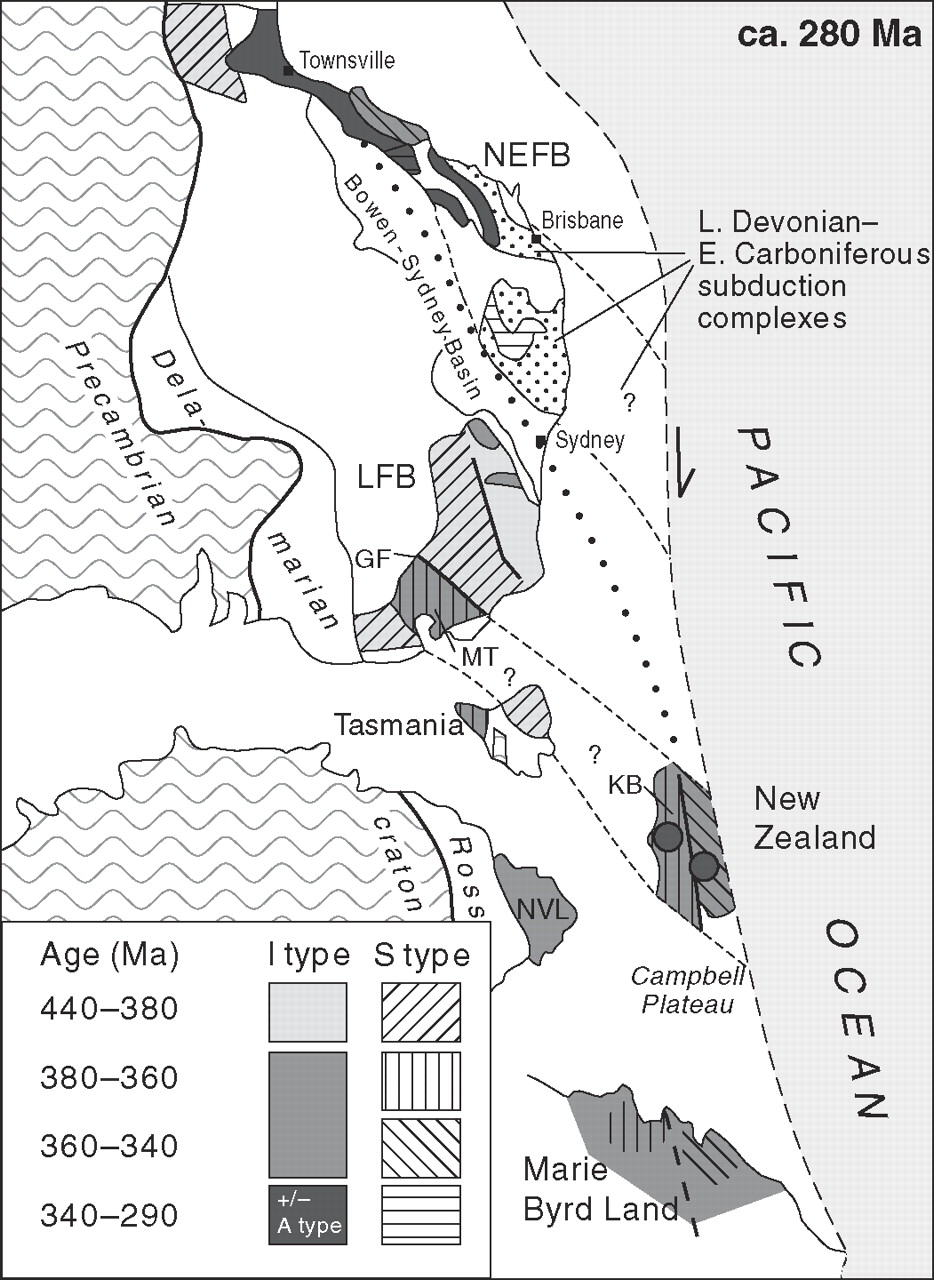
\includegraphics[width=1\textwidth]{Granite_Types_from_the_Eastern_Australian_Margin.jpg}
\caption{\label{fig:GraniteTypes} Granite Types from the Mesozoic Eastern Australian Margin}
\end{figure}

In most cases, granite plutons in Victoria fall neatly into being either S-type or I-type. Interestingly, there is a Devonian granite body in central Victoria at Cobaw, which is a rare example of a zoned intrusion, with a central hornblende bearing I-type granite, surrounded by a 1-6 km wide rim of cordierite-bearing S-type Pyalong Adamellite, \cite{waight2000fingerprinting}. They describe field observations at Cobaw supporting a model of simultaneous emplacement of contrasting but genetically related felsic magmas  \cite{waight2001geochemical}. In this model, invasion of hot I-type magma (with a mantle-derived magma component) into mid-crustal metasediments produced S-type magma. They note that K-Ar, Ar-Ar and SHRIMP U-Pb data support essentially simultaneous emplacement at 367 ± 2 Ma. Fermio (1984)

\section{Conclusion}

Granite can be classified by its source; Sedimentary (S-type) or Igneous (I-type). To determine the source both geochemical and petrological characteristics are used.
Another classification that can be used to classify granites is the magmatic temperature.

In Victoria, the granites are predominantly S-type to the west and I-type to the east. This is consistent with the model of the Lachlan Fold Belt accreting onto the older Gondwanan Craton to the west during the Benambran Orogeny which resulted in subsequent and widespread granite development in the Devonian.
\newpage


\bibliography{bibliography.bib}

\end{document}